%%%%%%%%%%%%%%%%%%%%%%%%%%%%%%%%%%%%%%%%%
% University/School Laboratory Report
% LaTeX Template
% Version 4.0 (March 21, 2022)
%
% This template originates from:
% https://www.LaTeXTemplates.com
%
% Authors:
% Vel (vel@latextemplates.com)
% Linux and Unix Users Group at Virginia Tech Wiki
%
% License:
% CC BY-NC-SA 4.0 (https://creativecommons.org/licenses/by-nc-sa/4.0/)
%
%%%%%%%%%%%%%%%%%%%%%%%%%%%%%%%%%%%%%%%%%

%----------------------------------------------------------------------------------------
%	PACKAGES AND DOCUMENT CONFIGURATIONS
%----------------------------------------------------------------------------------------

\documentclass[
	letterpaper, % Paper size, specify a4paper (A4) or letterpaper (US letter)
	10pt, % Default font size, specify 10pt, 11pt or 12pt
]{CSUniSchoolLabReport}

\addbibresource{sample.bib} % Bibliography file (located in the same folder as the template)

%----------------------------------------------------------------------------------------
%	REPORT INFORMATION
%----------------------------------------------------------------------------------------

\title{ECE 398-MA \\ Introduction to Modern Communication with Python and SDR \\ SDR Lab 1} % Report title

\author{Noah Breit} % Author name(s), add additional authors like: '\& James \textsc{Smith}'

\date{\today} % Date of the report

%----------------------------------------------------------------------------------------

\begin{document}

\maketitle % Insert the title, author and date using the information specified above

% \begin{center}
% 	\begin{tabular}{l r}
% 		Date Performed: & February 13, 2022 \\ % Date the experiment was performed
% 		Partners: & Cecilia \textsc{Smith} \\ % Partner names
% 		& Tajel \textsc{Khumalo} \\
% 		Instructor: & Professor \textsc{Rivera} % Instructor/supervisor
% 	\end{tabular}
% \end{center}

% If you need to include an abstract, uncomment the lines below
%\begin{abstract}
%	Abstract text
%\end{abstract}

%----------------------------------------------------------------------------------------
%	OBJECTIVE
%----------------------------------------------------------------------------------------

\section{Assignment 1}

\begin{figure}[H] % [H] forces the figure to be placed exactly where it appears in the text
	\centering % Horizontally center the figure
	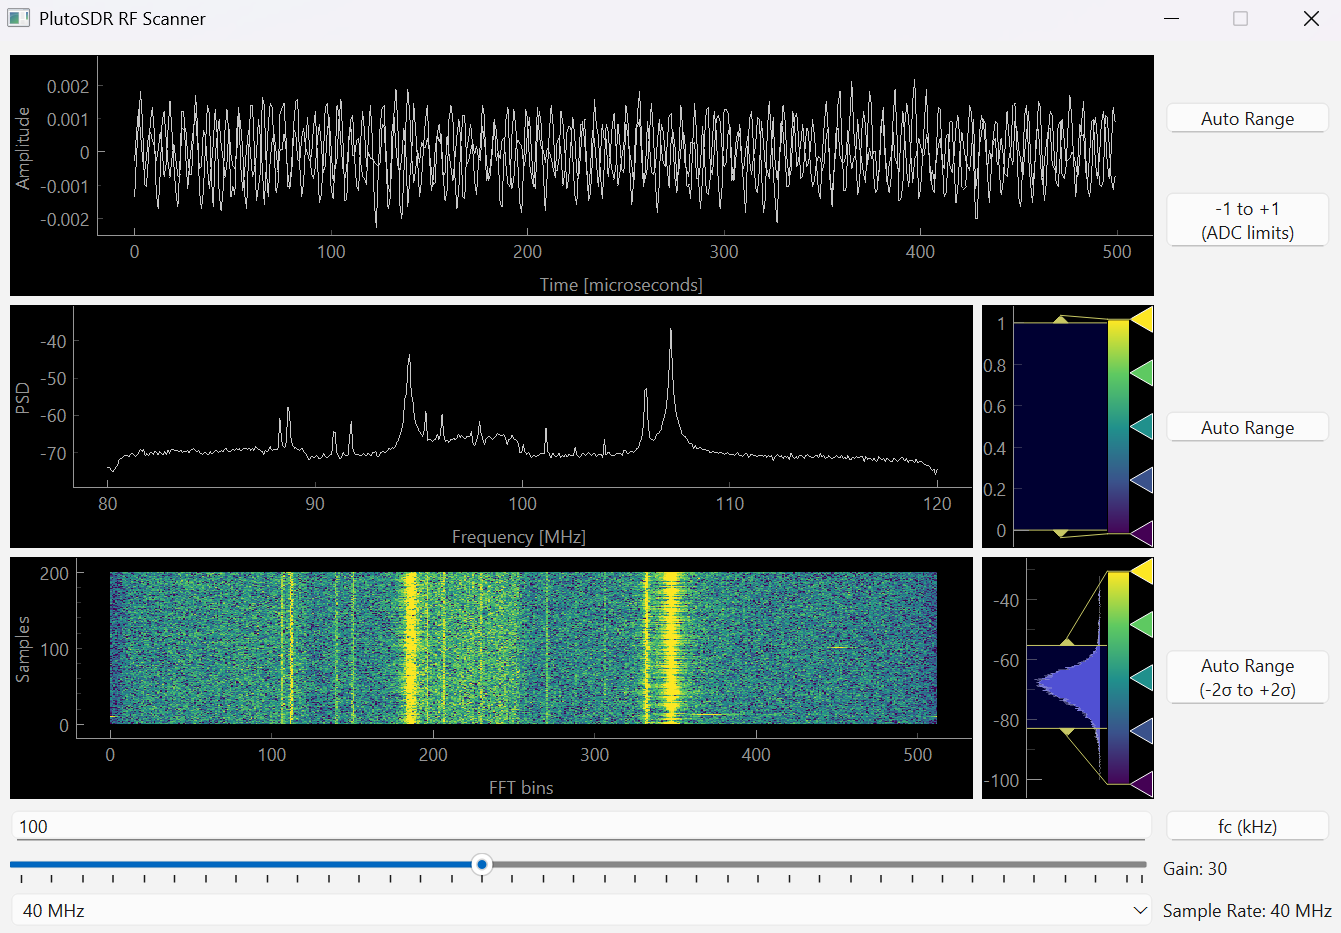
\includegraphics[width=1.2\textwidth]{assignment1a.png} % Include the figure
	\caption{RF Scanner GUI @ 100 MHz (FM BAND)}
	\label{fig:block}
\end{figure}

\begin{figure}[H] % [H] forces the figure to be placed exactly where it appears in the text
	\centering % Horizontally center the figure
	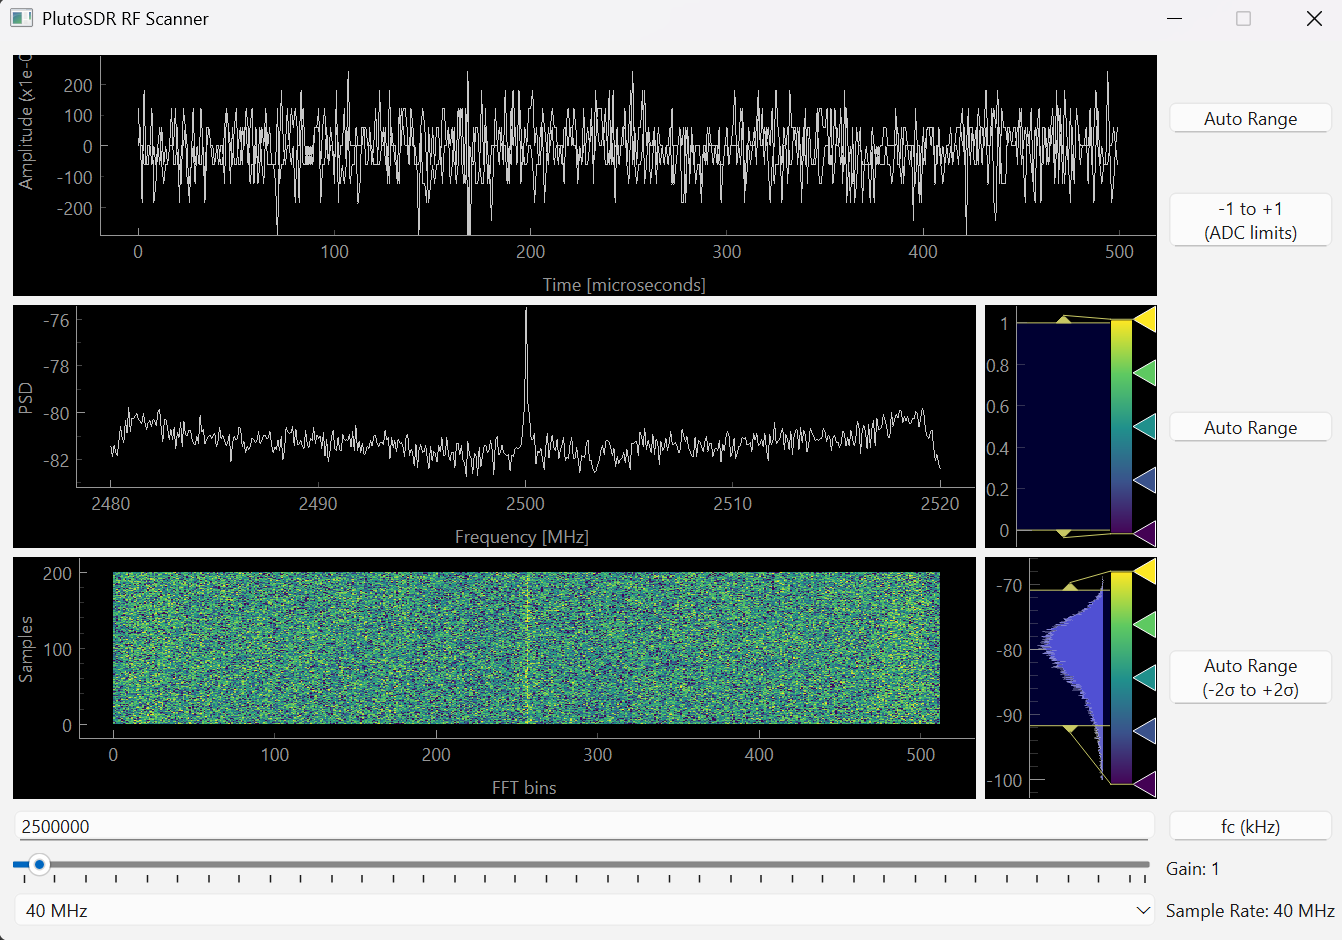
\includegraphics[width=1.2\textwidth]{assignment1b.png} % Include the figure
	\caption{RF Scanner GUI @ 2.5 GHz (WiFi BAND)}
	\label{fig:block}
\end{figure}

\section{Assignment 2}

\begin{figure}[H] % [H] forces the figure to be placed exactly where it appears in the text
	\centering % Horizontally center the figure
	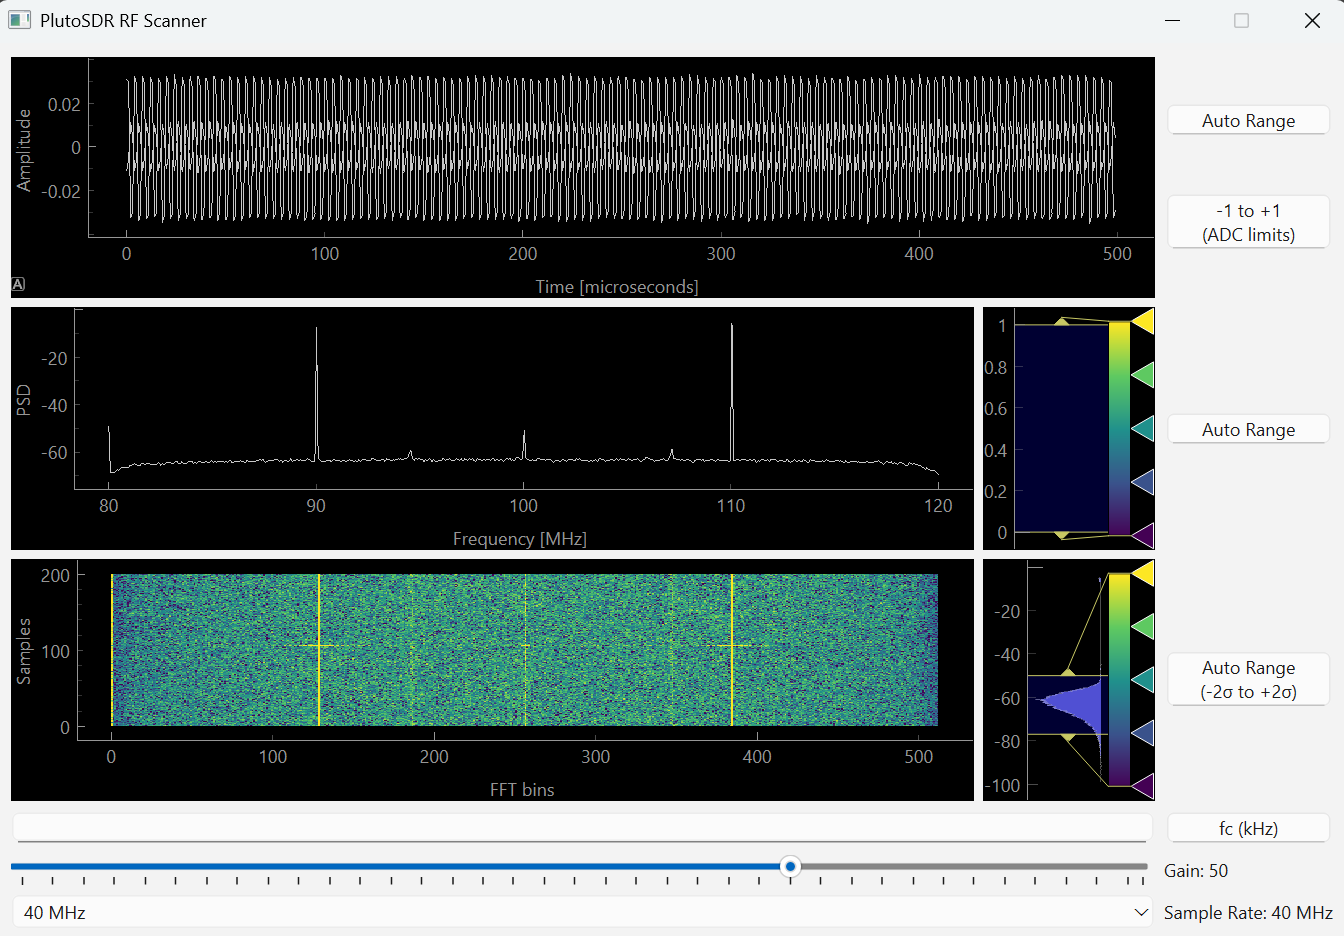
\includegraphics[width=1.2\textwidth]{assignment2a.png} % Include the figure
	\caption{Two Tone Signal @ 100 MHz}
	\label{fig:block}
\end{figure}

Two Tone Signal code provided below:
\begin{lstlisting}[language=Python]
	
	############ YOUR CODE STARTS HERE ############
	
	t = np.arange(0, Ns/sample_rate, 1/sample_rate)  # Time vector
	# Generate two-tone signal at baseband (hint: cosine already has two tones at f_tone and -f_tone)
	tx_samples = np.cos(2*np.pi*f_tone*t)   # Fc Carrier Freq @ 100 MHz, 
	# so freq components will appear at
	# 90 MHz and 110 MHz
	
	############ YOUR CODE STOPS HERE ############

\end{lstlisting}

\begin{figure}[H] % [H] forces the figure to be placed exactly where it appears in the text
	\centering % Horizontally center the figure
	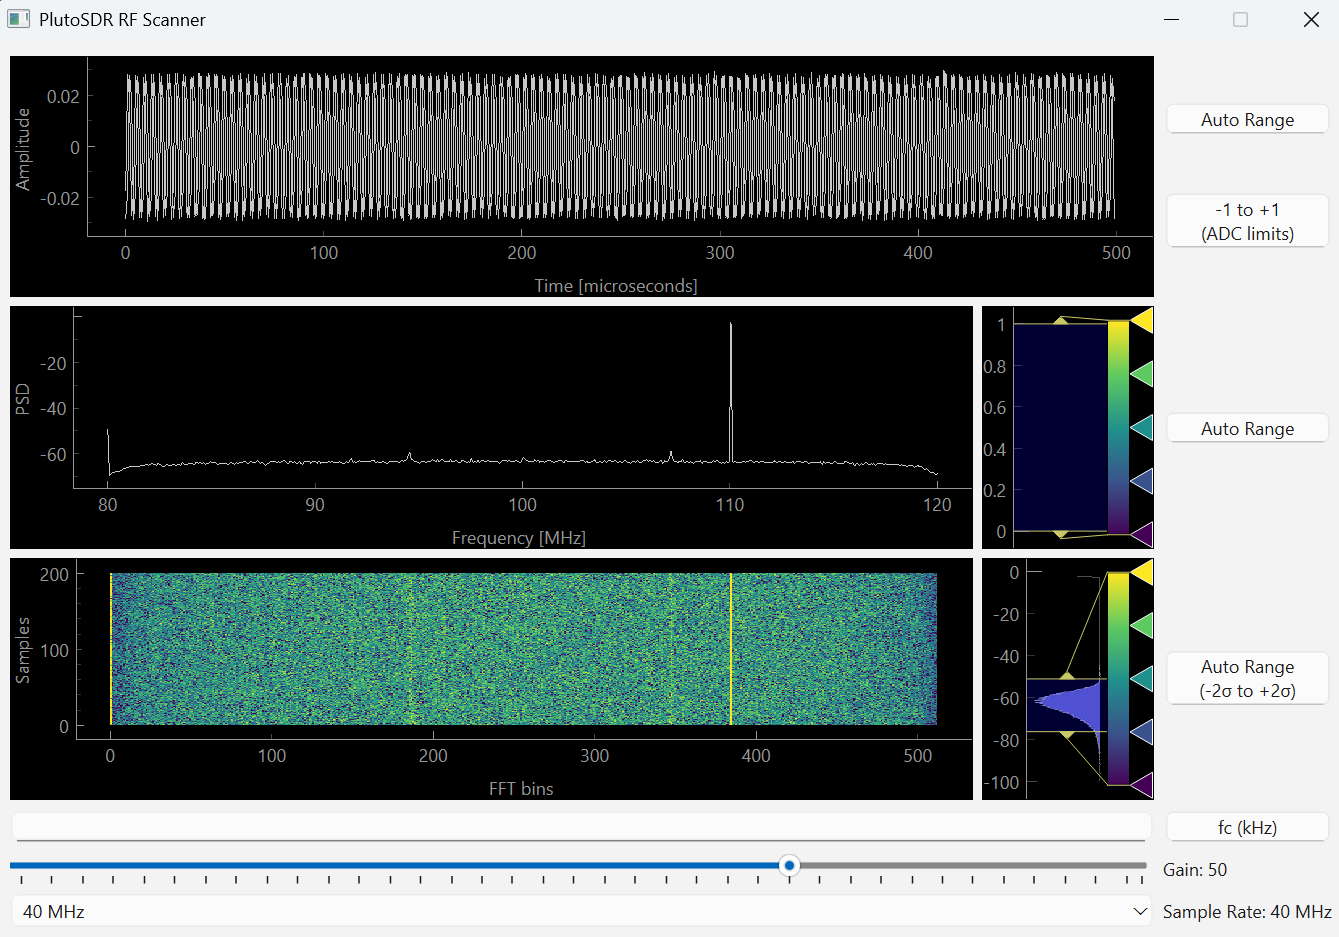
\includegraphics[width=1.2\textwidth]{assignment2b.png} % Include the figure
	\caption{Single Tone Signal @ 100 MHz}
	\label{fig:block}
\end{figure}

Single Tone Signal code provided below:
\begin{lstlisting}[language=Python]
	
	############ YOUR CODE STARTS HERE ############
	
	t = np.arange(0, Ns/sample_rate, 1/sample_rate)  # Time vector
	# Generate one-tone signal at baseband (110 MHz)
	tx_samples = np.exp(1j*2*np.pi*f_tone*t)    # Fc Carrier Freq @ 100 MHz, 
	# so freq components will appear at
	# 110 MHz
	
	############ YOUR CODE STOPS HERE ############
	
\end{lstlisting}

\begin{figure}[H] % [H] forces the figure to be placed exactly where it appears in the text
	\centering % Horizontally center the figure
	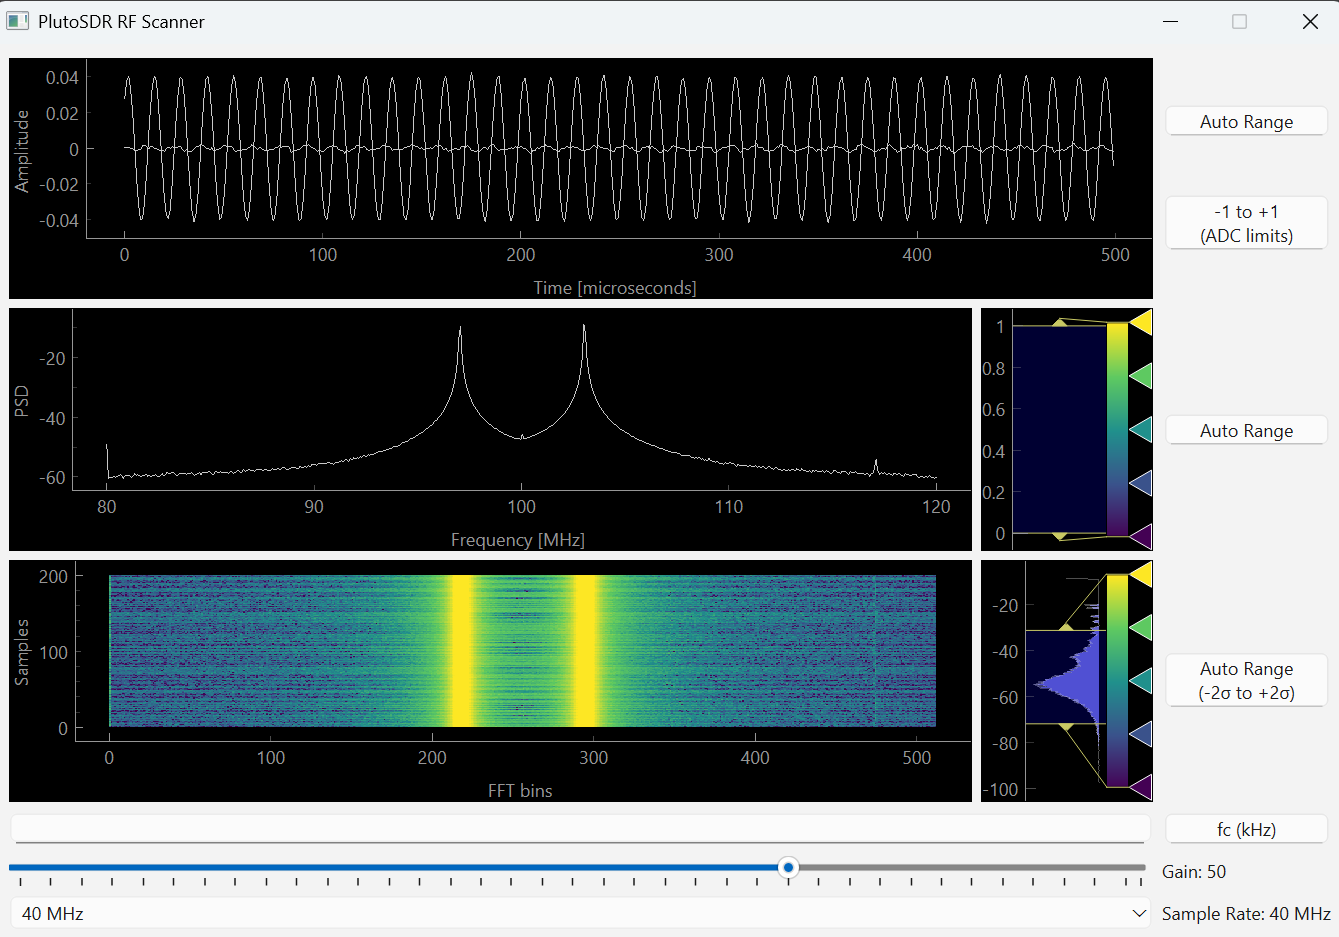
\includegraphics[width=1.2\textwidth]{assignment2c1.png} % Include the figure
	\caption{Two Tone Signal w 3 MHz f-tone @ 100 MHz}
	\label{fig:block}
\end{figure}

\begin{figure}[H] % [H] forces the figure to be placed exactly where it appears in the text
	\centering % Horizontally center the figure
	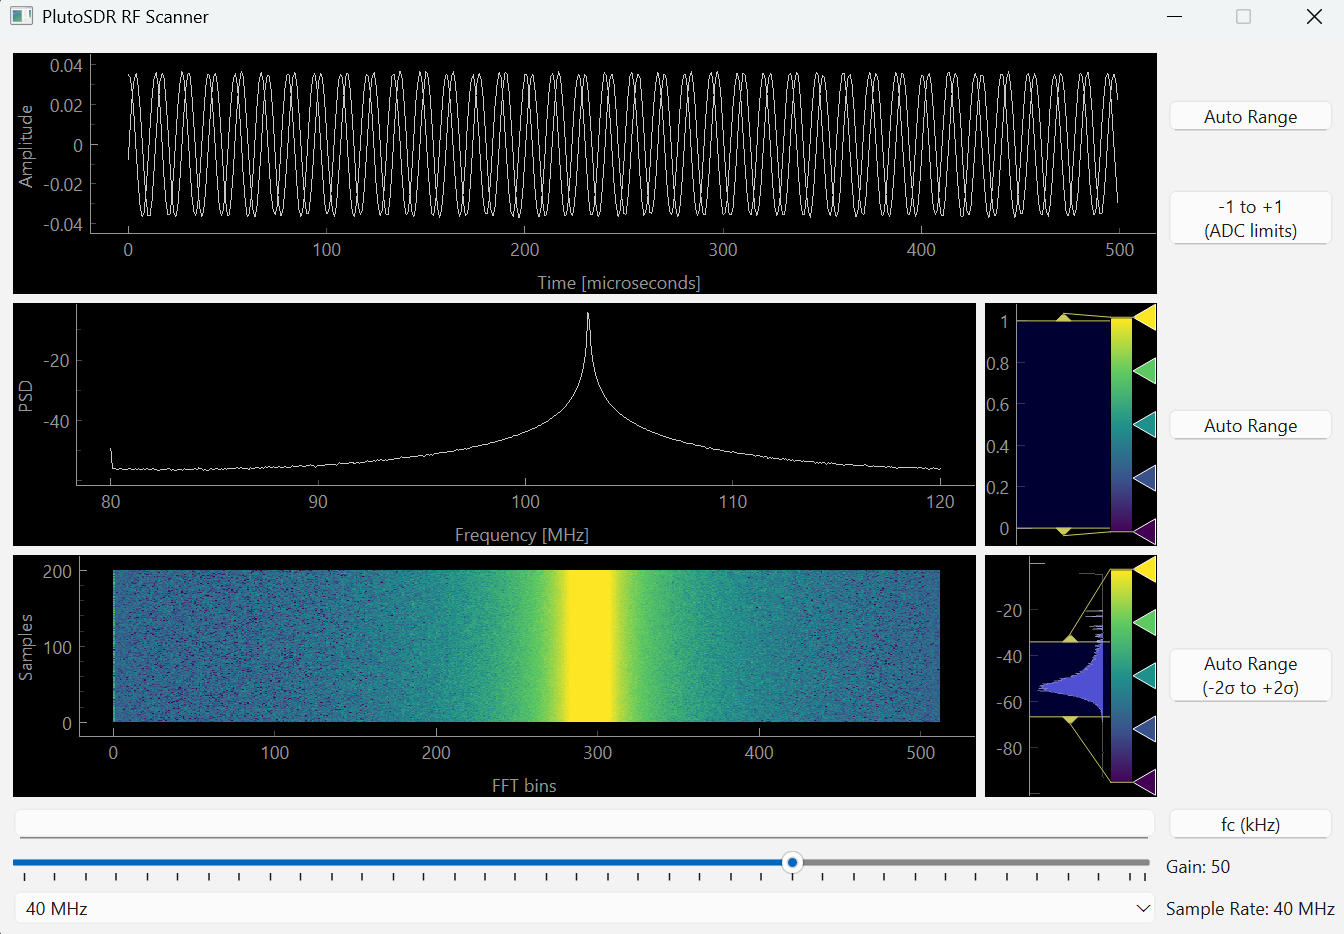
\includegraphics[width=1.2\textwidth]{assignment2c2.png} % Include the figure
	\caption{Single Tone Signal w 3 MHz f-tone @ 100 MHz}
	\label{fig:block}
\end{figure}

The spectrum changes when ‘f-tone’ is changed to 3 MHz because the bandwidth of the signal exceeds the 3 MHz ‘distance’ between the peaks of (+)f-tone and (-)f-tone frequency components. We know this because the spectrum analyzer shows that the region between the peaks at around 100 MHz is at -40 dB while the region above and below the peaks decreases to -60 dB.

\end{document}